\documentclass{article}%
\usepackage[T1]{fontenc}%
\usepackage[utf8]{inputenc}%
\usepackage{lmodern}%
\usepackage{textcomp}%
\usepackage{lastpage}%
\usepackage[tmargin=4cm,rmargin=2cm,lmargin=4cm,bmargin=3cm]{geometry}%
\usepackage[spanish]{babel}%
\usepackage[pages=all]{background}%
\backgroundsetup{placement=center,
 angle=0, scale=1, contents={
\includegraphics{Membrete.pdf}}, opacity=1}
%
\usepackage{ragged2e}%
\usepackage{xcolor}%
\usepackage{subcaption}%
\usepackage{graphicx}%
%
%
%
\begin{document}%
\normalsize%
\begin{center}%
\textcolor{white}{ 
HH
}%
\linebreak%
\linebreak%
\linebreak%
\linebreak%
\linebreak%
\linebreak%
\linebreak%
\linebreak%
\linebreak%
\linebreak%
\linebreak%
\linebreak%
\linebreak%
\linebreak%
\linebreak%
\begin{Huge}%
PROPUESTA DE VALOR PARA LA CONSTRUCCIÓN DE UNA HORNILLA%
\end{Huge}%
\linebreak%
\linebreak%
\linebreak%
\linebreak%
\linebreak%
\linebreak%
\linebreak%
\linebreak%
\linebreak%
\linebreak%
\begin{Large}%
Presentado por: AGROSAVIA%
\end{Large}%
\linebreak%
\begin{small}%
(Corporación Colombiana de Investigación Agropecuaria)%
\end{small}%
\end{center}%
\newpage%
\begin{large}%
 %
\textcolor{white}{ 
HH
}%
\linebreak%
Bogotá D.C., %
\ {\today}%
\newline%
 \newline%
%
\linebreak%
\newline%
Señor (es):%
\newline%
Nuevo\_usuario%
\newline%
Santander,  'Barbosa'.%
\newline%
 \newline%
%
\newline%
Apreciado(s) productor(es):%
\newline%
 \newline%
%
Con base en la información suministrada, está aplicación ha tasado (ver Sección 1) la construcción de una hornilla Plana CIMPA con capacidad de 106 kg/h; adecuada para el procesamiento de hasta 1.8 ha de caña, con un rendimiento de 216.0 T/mes y un periodo vegetativo de 10.0 meses. Teniendo en cuenta que se realizan 2 moliendas al mes se establece una tiene una jornada laboral de 6 días a la semana de 12 horas laborables cada una. \newline%
 Además, la aplicación estima que para garantizar una operación apropiada de la hornilla durante la producción de panela se requiere de un área (ver Sección 3) disponible de al menos 320 m² con una configuración de pailas y molino que garantiza una producción de panela de 50 toneladas al mes (ver Sección 2)%
, cuya productividad puede aumentar al incorporar el sistema de recuperación de calor como se muestra en las tablas del análisis financiero.%
\newline%
 Finalmente, está propuesta de valor se basa en condiciones del terreno ideales y estacionarias, por lo que, AGROSAVIA no se hace responsable de la reproducción total o parcial del material aquí suministrado sin una aprobación corporativa. No obstante, la corporación ofrece los siguientes servicios de asistencia técnica para ajustar los valores provistos en esta propuesta de valor:%
\begin{itemize}%
\item%
Estudio detallado para la construcción e instalación de la hornilla.%
\item%
Una visita técnica de dos funcionarios de AGROSAVIA para la puesta en marcha y capacitación de los operarios en el manejo de la hornilla y en la producción de panela saborizada, granulada o moldeada en presentación pastilla de chocolate.%
\item%
Entrega de un ejemplar de la guía tecnológica para el manejo integral del sistema productivo de la caña panelera y una para el mantenimiento de la hornilla.%
\end{itemize}%
Cualquier inquietud AGROSAVIA está presta a atenderla.\newline%
Cordial saludo.\newline%
\newline%
 \newline%
 \newline%
 \newline%
AGROSAVIA (Corporación colombiana de investigación agropecuaria)%
\end{large}%
\newpage%
\begin{large}%
 %
\begin{Large}%
\textbf{Contenido}%
\end{Large}%
\begin{itemize}%
\item%
Sección 1%
\begin{itemize}%
\item%
Información del usuario.%
\item%
Características de la caña sembrada.%
\item%
Características del molino.%
\item%
Análisis financiero.%
\end{itemize}%
\item%
Sección 2%
\begin{itemize}%
\item%
Diagramas mecánicos de las pailas.%
\item%
Diagramas mecánicos del recuperador de calor.%
\end{itemize}%
\item%
Sección 3%
\begin{itemize}%
\item%
Diagramas mecánicos de la chimenea.%
\item%
Diagramas mecánicos del ducto.%
\item%
Diagramas mecánicos de la chimenea.%
\item%
Diagramas mecánicos del proceso productivo.%
\end{itemize}%
\end{itemize}%
\end{large}%
\newpage%
\begin{center}%
\textcolor{white}{ 
HH
}%
\linebreak%
\linebreak%
\linebreak%
\linebreak%
\linebreak%
\linebreak%
\linebreak%
\linebreak%
\linebreak%
\linebreak%
\linebreak%
\linebreak%
\linebreak%
\linebreak%
\linebreak%
\begin{Huge}%
SECCIÓN 1:%
\end{Huge}%
\linebreak%
\begin{Huge}%
INFORMACIÓN TÉCNICA Y FINANCIERA%
\end{Huge}%
\end{center}%
\newpage%
\begin{center}%
\begin{Huge}%
DATOS DEL USUARIO%
\end{Huge}%
\linebreak%
\end{center}%
\begin{tabular}{lccccl}%
\textbf{Nombre de usuario}& & & & &Nuevo\_usuario\\%
\textbf{Correo}& & & & &Agro@Agro\\%
\textbf{Telefono}& & & & &1234567\\%
\textbf{Departamento}& & & & &Santander\\%
\textbf{Ciudad}& & & & & 'Barbosa'\\%
\textbf{Área caña sembrada}& & & & &18 ha\\%
\textbf{Crecimiento aproximado del área sembrada}& & & & &0 ha\\%
\textbf{Caña esperada por hectárea}& & & & &120 T/ha\\%
\textbf{Número de moliendas}& & & & &2 semanal(es)\\%
\textbf{Días de trabajo a la semana}& & & & &6\\%
\textbf{Horas de trabajo al día}& & & & &12\\%
\textbf{Cantidad de variedades de caña sembrada}& & & & &4\\%
\textbf{Altura media sobre el nivel del mar}& & & & &200 m\\%
\textbf{Nivel freático}& & & & &>100 m\\%
\textbf{Periodo vegetativo}& & & & &10.0 mes(es)\\%
\textbf{Grados Brix de la caña (promedio)}& & & & &18.975\\%
\textbf{Grados Brix de la panela (promedio)}& & & & &91.275\\%
\end{tabular}%
\newpage%
\begin{center}%
\begin{Huge}%
CARACTERÍSTICAS DE LAS VARIEDADES DE CAÑA SELECCIONADAS%
\end{Huge}%
\linebreak%
\end{center}%
\begin{tabular}{lcccccl}%
\textbf{Variedad de Caña 1}& & & & & &RD75{-}11\\%
\textbf{Grados Brix de la caña 1}& & & & & &19.2\\%
\textbf{pH}& & & & & &5.7\\%
\textbf{Azúcares reductores (\%)}& & & & & &0.9\\%
\textbf{Sacarosa (\%)}& & & & & &18.2\\%
\textbf{Pureza (\%)}& & & & & &94.8\\%
\textbf{Fósforo (ppm)}& & & & & &66\\%
\textbf{Grados Brix de la panela 1}& & & & & &90.8\\%
\end{tabular}%
\linebreak%
\newline%
%
\linebreak%
\begin{tabular}{lcccccl}%
\textbf{Variedad de Caña 2}& & & & & &POJ2878\\%
\textbf{Grados Brix de la caña 2}& & & & & &17.1\\%
\textbf{pH}& & & & & &5.3\\%
\textbf{Azúcares reductores (\%)}& & & & & &2.4\\%
\textbf{Sacarosa (\%)}& & & & & &14.1\\%
\textbf{Pureza (\%)}& & & & & &82.5\\%
\textbf{Fósforo (ppm)}& & & & & &168\\%
\textbf{Grados Brix de la panela 2}& & & & & &91.5\\%
\end{tabular}%
\linebreak%
\newline%
%
\linebreak%
\begin{tabular}{lcccccl}%
\textbf{Variedad de Caña 3}& & & & & &CP75{-}11\\%
\textbf{Grados Brix de la caña 3}& & & & & &20.4\\%
\textbf{pH}& & & & & &5.34\\%
\textbf{Azúcares reductores (\%)}& & & & & &1.5\\%
\textbf{Sacarosa (\%)}& & & & & &18.5\\%
\textbf{Pureza (\%)}& & & & & &90.7\\%
\textbf{Fósforo (ppm)}& & & & & &DESCONOCIDO\\%
\textbf{Grados Brix de la panela 3}& & & & & &92\\%
\end{tabular}%
\linebreak%
\newline%
%
\linebreak%
\begin{tabular}{lcccccl}%
\textbf{Variedad de Caña 4}& & & & & &RD75{-}11\\%
\textbf{Grados Brix de la caña 4}& & & & & &19.2\\%
\textbf{pH}& & & & & &5.7\\%
\textbf{Azúcares reductores (\%)}& & & & & &0.9\\%
\textbf{Sacarosa (\%)}& & & & & &18.2\\%
\textbf{Pureza (\%)}& & & & & &94.8\\%
\textbf{Fósforo (ppm)}& & & & & &66\\%
\textbf{Grados Brix de la panela 4}& & & & & &90.8\\%
\end{tabular}%
\linebreak%
\newline%
%
\linebreak%


\begin{figure}[h!]%
\begin{subfigure}{0.33\linewidth}%
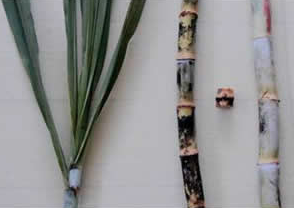
\includegraphics[width=0.95\linewidth]{Cana/RD75-11.png}%
\caption{Variedad de caña 1}%
\end{subfigure}%
\begin{subfigure}{0.33\linewidth}%
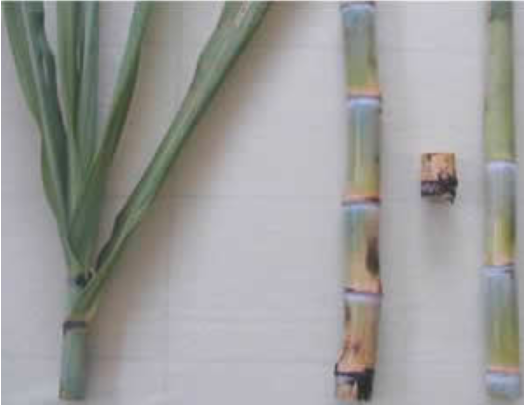
\includegraphics[width=0.95\linewidth]{Cana/POJ2878.png}%
\caption{Variedad de caña 2}%
\end{subfigure}%
\begin{subfigure}{0.33\linewidth}%
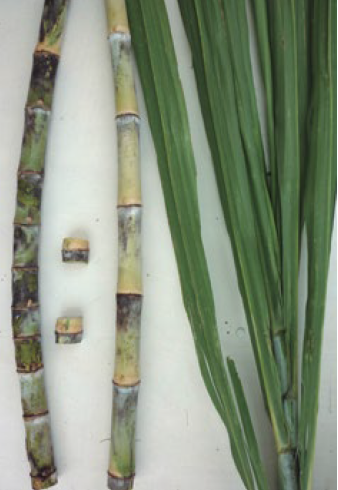
\includegraphics[width=0.95\linewidth]{Cana/CP75-11.png}%
\caption{Variedad de caña 3}%
\end{subfigure}%
\linebreak%
\newpage%
\end{figure}

%


\begin{figure}[h!]%
\begin{subfigure}{0.33\linewidth}%
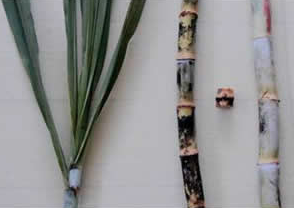
\includegraphics[width=0.95\linewidth]{Cana/RD75-11.png}%
\caption{Variedad de caña 4}%
\end{subfigure}%
\linebreak%
\newpage%
\end{figure}

%
\newpage%
\textcolor{white}{ 
HH
}%
\newpage%
\begin{center}%
\begin{Huge}%
MOLINOS PRESELECCIONADOS PARA ESTE DISEÑO%
\end{Huge}%
\linebreak%
\end{center}%
\begin{tabular}{lcccccl}%
\textcolor{red}{ 
\textbf{VALOR APROXIMADO DE UN MOLINO: }
}& & & & & &\textcolor{red}{ 
\$ 17,960,000.00
}\\%
\end{tabular}%
\linebreak%
\begin{tabular}{ccccc}%
MARCA&MODELO&KG POR HORA&DIESEL O GASOLINA (HP)&ELÉCTRICO (HP)\\%
&&&&\\%
HNReliable&HRJ{-}2000&2000&11&10\\%
JM Estrada&Trapiche 10 1{-}2&2000&16&18\\%
MIRACLE&MRC{-}EB2&2000&9&10\\%
Panelero&R14{-}AL&2000&25&20\\%
Panelero&R14{-}S&2000&25&20\\%
\linebreak%
\newline%
%
\linebreak%
\end{tabular}%


\begin{figure}[h!]%
\begin{subfigure}{0.33\linewidth}%
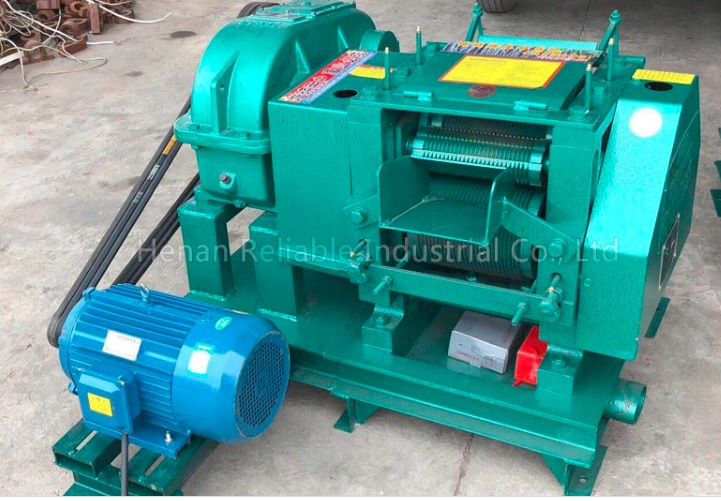
\includegraphics[width=0.95\linewidth]{Molinos/HRJ-2000.jpg}%
\caption{HRJ{-}2000}%
\end{subfigure}%
\begin{subfigure}{0.33\linewidth}%
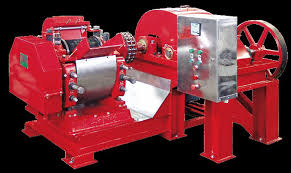
\includegraphics[width=0.95\linewidth]{Molinos/Trapiche 10 1-2.jpg}%
\caption{Trapiche 10 1{-}2}%
\end{subfigure}%
\begin{subfigure}{0.33\linewidth}%
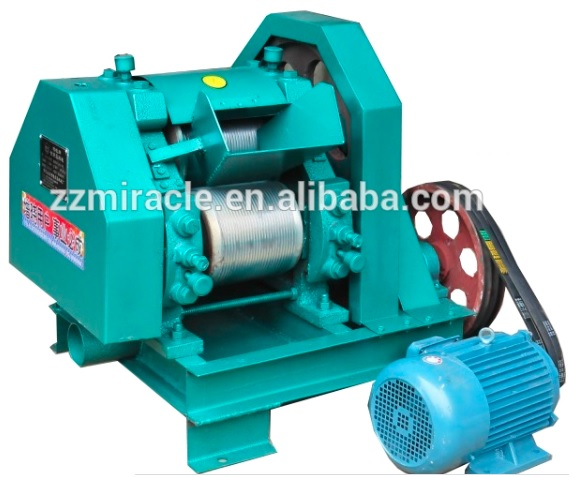
\includegraphics[width=0.95\linewidth]{Molinos/MRC-EB2.jpg}%
\caption{MRC{-}EB2}%
\end{subfigure}%
\linebreak%
\newpage%
\end{figure}

%


\begin{figure}[h!]%
\begin{subfigure}{0.33\linewidth}%
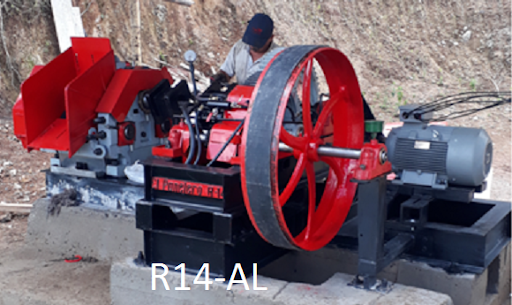
\includegraphics[width=0.95\linewidth]{Molinos/R14-AL.jpg}%
\caption{R14{-}AL}%
\end{subfigure}%
\begin{subfigure}{0.33\linewidth}%
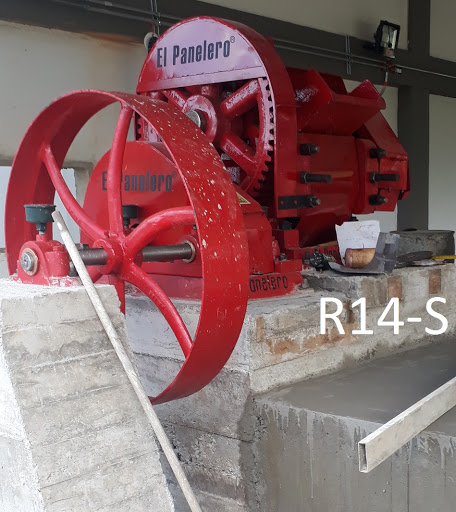
\includegraphics[width=0.95\linewidth]{Molinos/R14-S.jpg}%
\caption{R14{-}S}%
\end{subfigure}%
\linebreak%
\newpage%
\end{figure}

%
\newpage%
\textcolor{white}{ 
HH
}%
\newpage%
\end{document}